
\documentclass[plainboxedsections]{sciposter}

% A0 portrait dimensions
\setlength{\paperwidth}{33.1in}
\setlength{\paperheight}{46.8in}

\usepackage{mathpazo}
\usepackage{sourcecodepro}

\definecolor{BoxCol}{rgb}{1, 0.49, 0}
\definecolor{charlesBlue}{RGB}{100, 155, 255}
\definecolor{charlesBlueL}{RGB}{140, 195, 255}
\definecolor{SectionCol}{rgb}{1,1,1}

\usepackage[table, dvipsnames]{xcolor} 

\usepackage{amsmath}
\usepackage{amssymb}
\usepackage{multicol}
\usepackage{textcomp}

\usepackage{graphicx}
\usepackage{changepage}  % to adjust margins locally
\usepackage[framemethod=tikz]{mdframed}
\usepackage{centernot}
\renewcommand{\titlesize}{\fontsize{80}{20}}  %{\Huge} 
\renewcommand{\authorsize}{\fontsize{40}{20}} 
\renewcommand{\instsize}{\fontsize{30}{20}} 
\renewcommand{\sectionsize}{\Large}

\setmargins[4.5cm]

\newcommand{\highlight}[1]{%
  \colorbox{orange!50}{$\displaystyle#1$}}

\newcommand{\highlightB}[1]{%
  \colorbox{charlesBlueL}{$\displaystyle#1$}}

\makeatletter
\title{\titlesize\bfseries
  \vspace*{24pt}
  PCR TEST SENSITIVITY VS.\ TIME
}

\leftlogo[1.5]{img/flatiron-CCM-logo.png}
\rightlogo[0.75]{img/HSA-logo.png}

\author{
  \begin{center}
  \LARGE Bob Carpenter$^\dagger$ and Thomas Ward$^*$  \\
  \vspace*{12pt}
  \normalsize
  $^\dagger$Center for Computational Mathematics, Flatiron Institute, New York
  \\
  $^*$Joint Biosecurity Centre, UK Health Security Agency, London
  \vspace*{-48pt}
  \end{center}
} 

\begin{document}
\conference{\Large \null\hfill {\slshape International Society for Bayesian Analysis} (ISBA), World Meeting, July 2024, Venice}

\setlength{\fboxrule}{6pt}
\setlength{\fboxsep}{9pt}
% \fcolorbox{orange}{white}{
    \maketitle
    \hspace*{-1in}
% }
{\hrule height 4pt}
\hrule
\vspace*{12pt}
\begin{multicols}{2}
\begin{mdframed}[hidealllines = true, backgroundcolor = Cerulean!10]
{\large
\textbf{BACKGROUND:} From peak sensitivity at Covid symptom onset,
polymerase chain-reaction (PCR) test sensitivity declines over time.
\\[12pt]
Sensitivity is probability of positive test given a patient has Covid.
\\[24pt]
\textbf{GOAL:} Develop a Bayesian model to estimate sensitivity vs.\ time.
\\[24pt]
\textbf{FINDINGS:}
\begin{itemize}
\item {\bfseries Mixed population:} The fits suggest patients had mixture of short and long Covid.fit
\item {\bfseries Pharmacokinetics:} Log regression is solution to one-compartment clearance model, with mixture for two populations.
\end{itemize}
\vspace*{18pt}
\textbf{APPLICATIONS:}
\begin{itemize}
\item {\bfseries Estimating prevalence} from tests,
\item {\bfseries Estimating viral load} over time, and
\item {\bfseries Calibrating test surveys} with time-to-hospitalization,
  time-to-death, and post-stratification.
\end{itemize}
}
\end{mdframed}

\section{Data}

The data was collected from all patients admitted to one UK hospital with
Covid in mid-2020.  

\begin{center}
  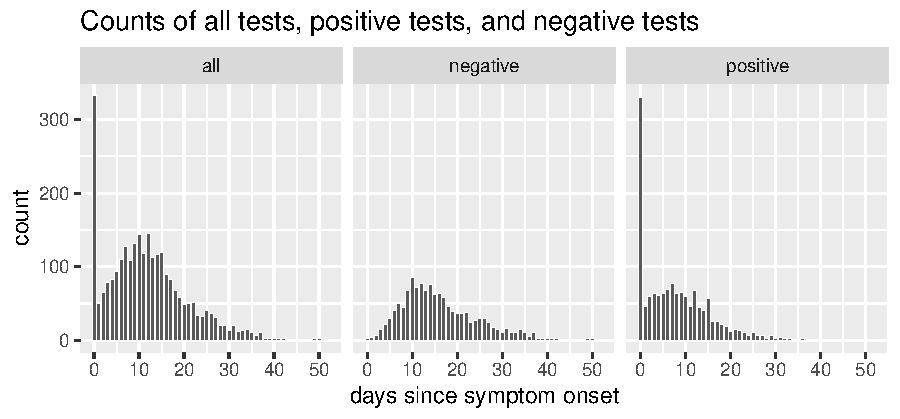
\includegraphics[width=0.47\textwidth]{img/data-counts.pdf}
\end{center}

{\small Sue Mallet et al. (2020) ``At what times during infection is SARS-CoV-2 detectable and no longer detectable using RT-PCR-based tests?'' {\slshape BMC Medicine}}

\section{Unconstrained MLE with standard errors}

% Independent maximum likelihood estimates with $\pm 1$ standard error bars.

\begin{center}
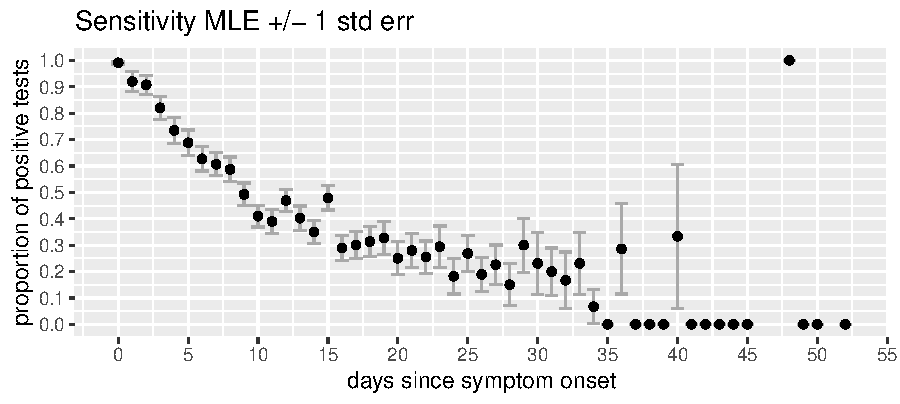
\includegraphics[width=0.475\textwidth]{img/mle.pdf}
\end{center}

\columnbreak

\section{Bayesian models}
\newcommand{\ilogit}{\textrm{logit}^{-1}}

{\bfseries Hetero (logit):} \
$y_n \sim \textrm{bernoulli}(\ilogit(\theta_{t_n}));
\quad \theta_t \sim 
\textrm{normal}(0, 3);
\quad \theta_{t+1} < \theta_t$
\\[12pt]
{\bfseries Hetero (log):} \
$y_n \sim \textrm{bernoulli}(\exp(\theta_{t_n}));
\quad \theta_t \sim \textrm{normal}(0, 3);
\quad \theta_{t+1} < \theta_t < 0$
%
\\ \hrule \mbox{}\\[6pt]
%
{\bfseries RW(1) (logit):} \
$y_n \sim \textrm{bernoulli}(\ilogit(\theta_{t_n}));
\quad \theta_{t+1} \sim \textrm{normal}(\theta_t, \sigma);
\quad \sigma \sim \textrm{normal}(0, 1);$
\\[2pt]
\null\qquad\qquad\qquad\qquad $\theta_{t+1} < \theta_t; 
\quad \sigma > 0$
\\[12pt]
{\bfseries RW(1) (log):} \
$y_n \sim \textrm{bernoulli}(\exp(\theta_{t_n}));
\quad \theta_{t+1} \sim \textrm{normal}(\theta_t, \sigma);
\quad \sigma \sim \textrm{normal}(0, 1);$
\\[2pt]
\null\qquad\qquad\qquad\qquad $\theta_{t+1} < \theta_t < 0;
\quad \sigma > 0$
%
\\ \hrule \mbox{}\\[6pt]
%
{\bfseries RW(2) (logit):} \
$y_n \sim \textrm{bernoulli}(\ilogit(\theta_{t_n})); 
\quad \theta_{t+2} \sim \textrm{normal}(\theta_{t-1} + (\theta_{t-1} - \theta_{t-2}), \sigma);$
\\[2pt]
\null\qquad\qquad\qquad\qquad $\sigma \sim \textrm{normal}(0, 0.5); 
\quad \theta_{t+1} < \theta_t; 
\quad \sigma > 0$
\\[12pt]
{\bfseries RW(2) (log):} \
$y_n \sim \textrm{bernoulli}(\exp(\theta_{t_n})); 
\quad \theta_{t+2} \sim \textrm{normal}(\theta_{t-1} + (\theta_{t-1} - \theta_{t-2}), \sigma);$
\\[2pt]
\null\qquad\qquad\qquad\qquad $\sigma \sim \textrm{normal}(0, 0.5); 
\quad \theta_{t+1} < \theta_t < 0; 
\quad \sigma > 0$
%
\\ \hrule \mbox{}\\[6pt]
%
{\bfseries Regression (logit):} \
$y_n \sim \textrm{bernoulli}(\ilogit(\alpha + \beta \cdot t_n));
\quad \alpha, \beta \sim \textrm{normal}(0, 0.5);
\quad \beta < 0$
\\[12pt]
{\bfseries Regression (log):} \
$y_n \sim \textrm{bernoulli}(\exp(\alpha + \beta \cdot t_n));
\quad \alpha, \beta \sim \textrm{normal}(0, 0.5); \quad \alpha, \beta < 0$
%
\\ \hrule \mbox{}\\[6pt]
%
{\bfseries Regress.\ mix (logit):}
$y_n \sim \textrm{bernoulli}(\lambda \cdot \ilogit(\alpha_1 + \beta_1 \cdot t_n) + (1 - \lambda) \cdot \ilogit(\alpha_2 + \beta_2 \cdot t_n)))$
\\[2pt]
\null\qquad\qquad\qquad\qquad $\lambda \sim \textrm{beta}(2, 2); 
\quad \alpha_k, \beta_k \sim \textrm{normal}(0, 1); 
\quad \beta_k < 0$
\\[12pt]
{\bfseries Regress.\ mix (logit):}
$y_n \sim \textrm{bernoulli}(\lambda \cdot \exp(\alpha_1 + \beta_1 \cdot t_n) + (1 - \lambda) \cdot \exp(\alpha_2 + \beta_2 \cdot t_n))$
\\[2pt]
\null\qquad\qquad\qquad\qquad $\lambda \sim \textrm{beta}(2, 2); 
\quad \alpha_k, \beta_k \sim \textrm{normal}(0, 1); 
\quad \alpha_k, \beta_k < 0.$



\section{Model comparison regression fit}

Approximate leave-one-out cross-validation estimates of expected log
predictive density (ELPD) differences plus standard
errors of differences.  Estimated using Stan's \texttt{loo} package.
\vspace*{12pt}
\begin{center}
\renewcommand{\arraystretch}{1.4}
\begin{tabular}{ll|rr}
\hline
Model & Scale & ELPD (diff) & standard error (diff)
\\ \hline
2nd-order random walk & \ log &  0.0 & 0.0
\\
Regression mixture & \ log &   -0.4 &      1.5  
\\
1st-order random walk & \ log        &         -0.9 &       0.7  
\\
Regression & \ log &   -2.8  &     2.7  
\\
Heterogeneous & \ log & -3.0     &  1.8  
\\ \hline
Heterogeneous & \ logit &    -3.0    &   1.9  
\\
2nd-order random walk & \ logit  & -6.7     &  3.7  
\\
1st-order random walk & \ logit              & -8.4      & 3.8  
\\
Regression mixture & \ logit  & -15.0  &     4.1  
\\
Regression & \ logit & -81.6   &    9.9
\\ \hline
\end{tabular}

\section{Log (mixture) regression coefficient estimates}

{\bf Regression (log)}: $\widehat{\alpha} = -0.01; \quad \widehat{\beta} =
-0.07$ \hfill \null
\\[4pt]
{\bf Regression (log mix):} $\widehat{\alpha}_1 = -0.02; \ \widehat{\beta}_1 = -0.04; \quad
\widehat{\alpha}_2 = -0.03; \ \widehat{\beta}_2 = -0.18; \quad \widehat{\lambda} = 0.6$ \hfill \null

% log mixture: alpha1 = -.02;  alpha2 = -.03;
%              beta1 = -0.04, beta2 = -.18
%              phi = 0.6
% single component, alpha = -0.01, beta = -0.07


\section{Reproducible GitHub repository}
\null \hfill

\includegraphics[width=0.0825\textwidth]{img/qr-code.pdf}
\hfill

\includegraphics[width=0.065\textwidth]{img/stan-logo.png}
\hfill \null
\\
\texttt{https://github.com/bob-carpenter/pcr-sensitivity-vs-time}
\end{center}
\end{multicols}


\section{Visual model comparison}
  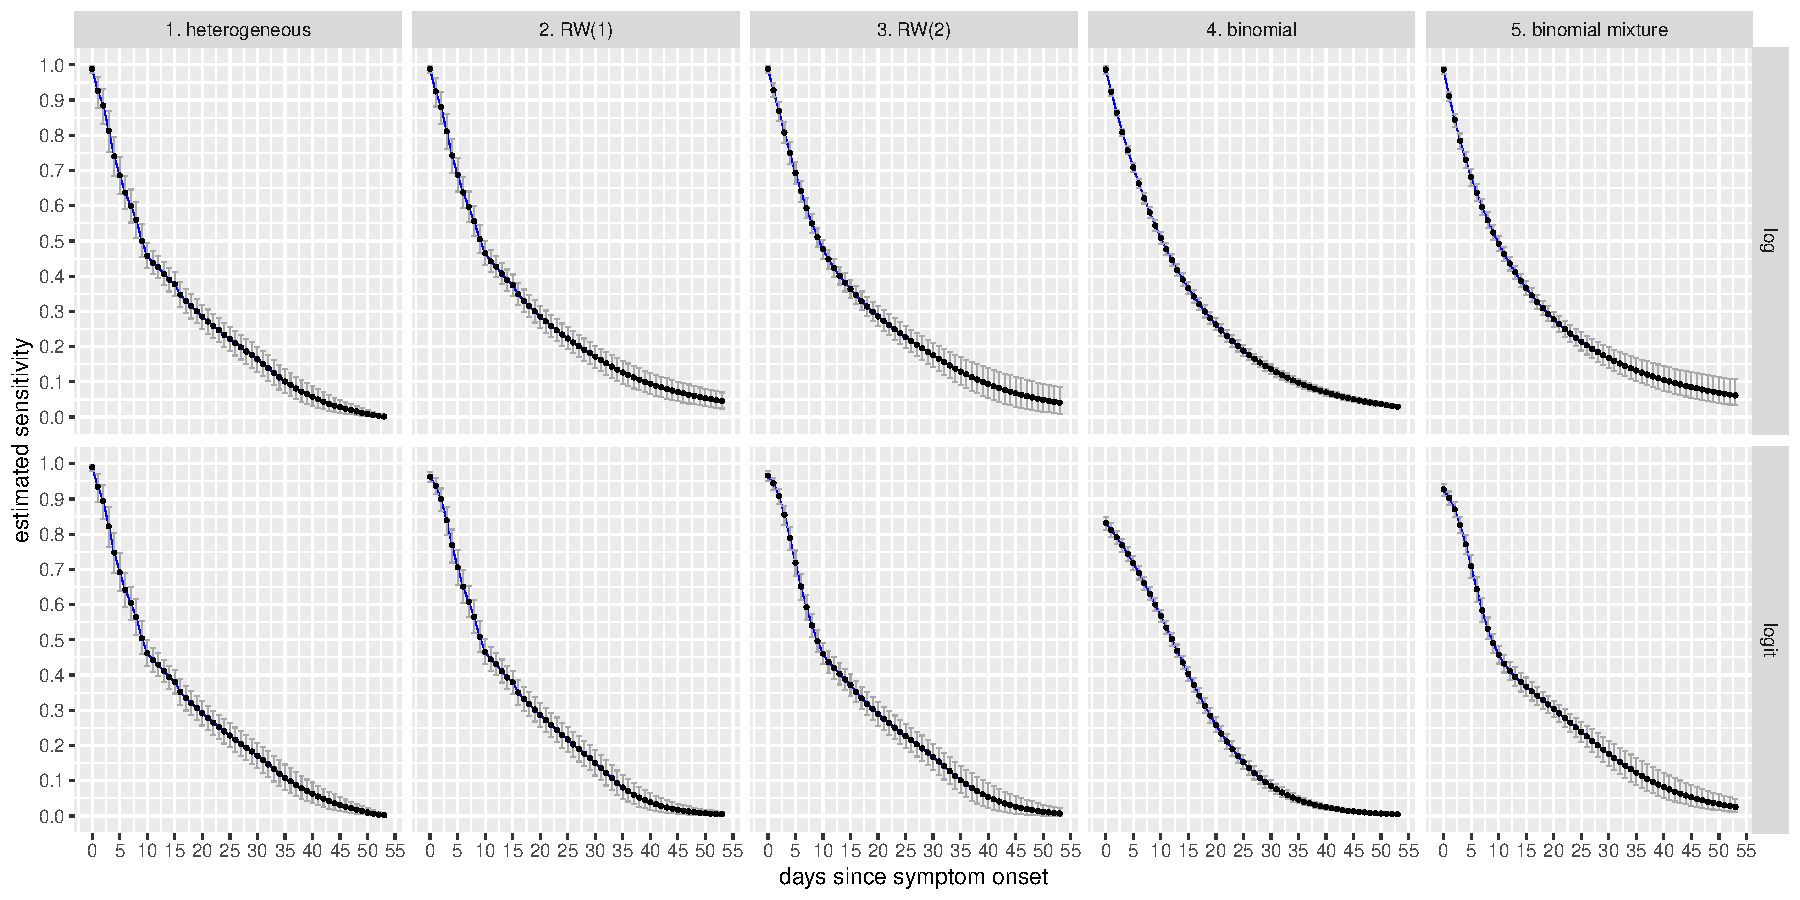
\includegraphics[width=\textwidth]{img/model-link-comparison.pdf}
\end{document}

